\subsection{Entity-Relationship Schema}

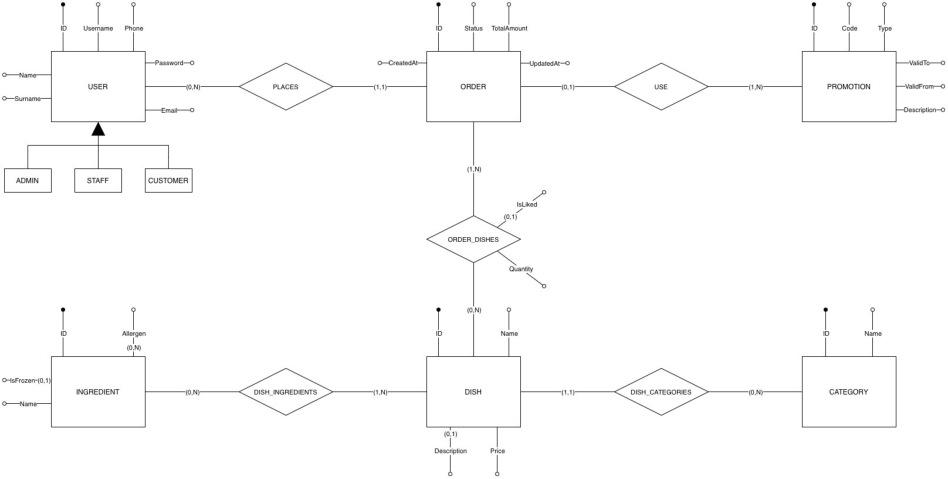
\includegraphics[]{images/ERSchema.pdf}

The enumerated domains used by the schema:
\begin{itemize}
    \item \texttt{USER\_ROLE} is used by \texttt{users.role}, it is mandatory and it restricts the allowed values to \texttt{STAFF}, \texttt{CUSTOMER}, and \texttt{ADMIN}.
    \item \texttt{ORDER\_STATUS} is used by \texttt{orders.status}, it is also mandatory, and it restricts the allowed values to \texttt{PENDING}, \texttt{COMPLETED}, and \texttt{CANCELLED}.
    \item \texttt{ALLERGEN} is the domain used inside the array attribute \texttt{ingredients.allergen}, and it enumerates the allergen categories supported by the application.
\end{itemize}

We have 8 tables in the schema, including the associative entities introduced by the relational design:

\begin{itemize}
    \item \textbf{User (\texttt{users})}: each user is defined by \texttt{id}, which is of type \texttt{SERIAL}, mandatory, and is the primary key of the entity. Then we have \texttt{username}, of type \texttt{VARCHAR(20)}, which is mandatory and unique, and stores the public username chosen by the user. We also have \texttt{email}, of type \texttt{VARCHAR(255)}, mandatory and unique, which stores the email address associated with the account. The attributes \texttt{name} and \texttt{surname} are both of type \texttt{VARCHAR(255)}, both mandatory, and they store the user's first name and last name respectively. The attribute \texttt{phone\_number} is of type \texttt{VARCHAR(25)}, it is mandatory and unique, and it stores the phone number associated with the account. The attribute \texttt{role} is of type \texttt{USER\_ROLE}, it is mandatory, and it represents the logical role of the user inside the application. The attribute \texttt{password\_hash} is of type \texttt{VARCHAR(255)}, it is mandatory, and it stores the hashed password used for authentication. In the current schema, customers, staff members, and administrators are not modeled as separate entities, but are distinguished through the value of \texttt{role}.
    % TODO: capire se su CREATE.sql è sensato avere type in promotion
    \item \textbf{Promotion (\texttt{promotions})}: each promotion is defined by \texttt{id}, which is of type \texttt{SERIAL}, mandatory, and is the primary key of the entity. Then we have \texttt{code}, of type \texttt{VARCHAR(20)}, which is mandatory and unique, and stores the promotion code that can be applied to an order. The attribute \texttt{type} is of type \texttt{VARCHAR(20)}, it is mandatory, and it stores the type of promotion; in the current implementation it is free text, even if a future enum could make the domain more explicit. The attribute \texttt{description} is of type \texttt{VARCHAR(20)}, it is mandatory and it stores a short textual description of the promotion. Finally, \texttt{valid\_from} and \texttt{valid\_to} are both of type \texttt{TIMESTAMP}, both mandatory, and they store the beginning and the end of the validity interval of the promotion respectively. Moreover, the relational schema enforces the constraint \texttt{valid\_to > valid\_from}, so the ending time of the promotion must always be later than its starting time.

    \item \textbf{Order (\texttt{orders})}: each order is defined by \texttt{id}, which is of type \texttt{SERIAL}, mandatory, and is the primary key of the entity. Then we have \texttt{user\_id}, of type \texttt{INTEGER}, which is mandatory and is a foreign key toward \texttt{users(id)} with \texttt{ON DELETE CASCADE}; it identifies the user who placed the order. The attribute \texttt{promotion\_id} is of type \texttt{INTEGER}, it is optional, and it is a foreign key toward \texttt{promotions(id)} with \texttt{ON DELETE SET NULL}; it identifies the promotion applied to the order, if any. The attribute \texttt{total\_amount} is of type \texttt{DECIMAL(10, 2)}, it is mandatory, and it stores the total monetary amount of the order. The attribute \texttt{status} is of type \texttt{ORDER\_STATUS}, it is mandatory, it defaults to \texttt{PENDING}, and it represents the current state of the order. In conclusion, \texttt{created\_at} and \texttt{updated\_at} are both of type \texttt{TIMESTAMP WITH TIME ZONE}, both mandatory, and both initialized with the current timestamp. The attribute \texttt{updated\_at} is also maintained by the \texttt{orders\_set\_updated\_at} trigger before each update. Finally, the pair \texttt{(user\_id, promotion\_id)} is constrained to be unique when a promotion is referenced.

    \item \textbf{Category (\texttt{categories})}: each category is defined only by \texttt{name}, which is of type \texttt{VARCHAR(255)}, mandatory, unique, and is the primary key of the entity; in the current relational schema, therefore, the category name itself identifies the record and no numeric identifier is used.

    \item \textbf{Dish (\texttt{dishes})}: each dish is defined by \texttt{id}, which is of type \texttt{SERIAL}, mandatory, and is the primary key of the entity. Then we have \texttt{name}, of type \texttt{VARCHAR(255)}, which is mandatory and stores the commercial name of the dish. The attribute \texttt{description} is of type \texttt{TEXT}, it is optional, and it stores an extended textual description of the dish. The attribute \texttt{category\_name} is of type \texttt{VARCHAR(255)}, it is mandatory, and it is a foreign key toward \texttt{categories(name)}; it identifies the category to which the dish belongs. The attribute \texttt{price} is of type \texttt{DECIMAL(10, 2)}, it is mandatory, and it stores the current price of the dish.

    \item \textbf{OrderDish (\texttt{order\_dishes})}: this associative entity represents the many-to-many relationship between orders and dishes. Each row is defined by \texttt{id}, which is of type \texttt{SERIAL}, mandatory, and is the primary key of the entity. Then we have \texttt{order\_id}, of type \texttt{INTEGER}, which is mandatory and is a foreign key toward \texttt{orders(id)} with \texttt{ON DELETE CASCADE}; it identifies the order to which the row belongs. We also have \texttt{dish\_id}, of type \texttt{INTEGER}, which is mandatory and is a foreign key toward \texttt{dishes(id)}; it identifies the ordered dish. The attribute \texttt{quantity} is of type \texttt{INTEGER}, it is mandatory, and it stores how many units of the dish are included in the order. Finally, \texttt{is\_liked} is of type \texttt{BOOLEAN}, it is optional, and it stores feedback on the ordered dish: \texttt{TRUE} means that the dish was liked, \texttt{FALSE} means that it was disliked, and \texttt{NULL} means that no feedback has been provided yet. The pair \texttt{(order\_id, dish\_id)} is constrained to be unique, so the same dish can appear at most once in the same order.

    \item \textbf{Ingredient (\texttt{ingredients})}: each ingredient is defined by \texttt{id}, which is of type \texttt{SERIAL}, mandatory, and is the primary key of the entity. Then we have \texttt{name}, of type \texttt{VARCHAR(255)}, which is mandatory and stores the ingredient name. The attribute \texttt{allergen} is of type \texttt{ALLERGEN[]}, it is optional, and it stores the list of allergens associated with the ingredient; the attribute may be null if no allergen information is stored for that ingredient. The attribute \texttt{is\_frozen} is of type \texttt{BOOLEAN}, it is optional, and it indicates whether the ingredient is frozen.

    \item \textbf{DishIngredient (\texttt{dish\_ingredients})}: this associative entity represents the many-to-many relationship between dishes and ingredients. Each row is defined by \texttt{id}, which is of type \texttt{SERIAL}, mandatory, and is the primary key of the entity. Then we have \texttt{dish\_id}, of type \texttt{INTEGER}, which is mandatory and is a foreign key toward \texttt{dishes(id)} with \texttt{ON DELETE CASCADE}; it identifies the dish. Finally, \texttt{ingredient\_id} is of type \texttt{INTEGER}, it is mandatory and is a foreign key toward \texttt{ingredients(id)} with \texttt{ON DELETE CASCADE}; it identifies the ingredient used in the dish. The pair \texttt{(dish\_id, ingredient\_id)} is constrained to be unique, so the same ingredient cannot be associated with the same dish more than once.
\end{itemize}

% TODO: non so se ha senso inserirla devo rifletterci.
The relationships represented by the current schema can be summarized as follows. A user can place many orders, while each order is associated with exactly one user through \texttt{orders.user\_id}. A promotion can be used by many orders, while each order can reference at most one promotion through \texttt{orders.promotion\_id}; the relational schema also enforces that the same non-null pair \texttt{(user\_id, promotion\_id)} cannot be repeated. Each dish belongs to exactly one category through \texttt{dishes.category\_name}, while each category can be associated with many dishes. Orders and dishes are connected by a many-to-many relationship implemented through \texttt{order\_dishes}, and this associative entity also stores relationship-specific information such as \texttt{quantity} and \texttt{is\_liked}. Dishes and ingredients are connected by a many-to-many relationship implemented through \texttt{dish\_ingredients}.
